\documentclass[11pt]{amsart}
%%%%%%%%%%%%%% Packages
\usepackage{amssymb,amsfonts,amsthm,amsmath}
\usepackage[english]{babel}
\usepackage[all,cmtip]{xy}
\usepackage{tikz}
\usepackage{mathtools}
\usepackage{tensor}
\usepackage{csquotes}
\usepackage[vcentermath]{youngtab}
%\usepackage{stix}
\usetikzlibrary{arrows,chains,matrix,positioning,scopes}
%\usepackage{mathrsfs}
%\usepackage[notcite,notref]{showkeys}


%%%%%%%%%%% Tikz
\makeatletter
\tikzset{join/.code=\tikzset{after node path={%
\ifx\tikzchainprevious\pgfutil@empty\else(\tikzchainprevious)%
edge[every join]#1(\tikzchaincurrent)\fi}}}
\makeatother
\tikzset{>=stealth',every on chain/.append style={join},
         every join/.style={->}}

        

%%%%%%%%%%%% Personalized commands and environments

\newcommand{\inputc}[1]{ \raisebox{-0.5\height}{\input{#1}} }
\newtheorem{theorem}{Theorem}
\newtheorem{lemma}[theorem]{Lemma}
\newtheorem{corollary}[theorem]{Corollary}
\newtheorem{definition}[theorem]{Definition}
\newtheorem{proposition}[theorem]{Proposition}
\newtheorem{remark}[theorem]{Remark}
\newtheorem{example}{Example}
%\newtheorem{theorem*}{Theorem}

\newcommand{\func}[3]{{#1} : {#2} \longrightarrow {#3}}
\numberwithin{equation}{section}
\newcommand{\dbar}{\bar{\partial}}
\newenvironment{myproof}{\noindent{it Proof}
\setlength{\parindent}{0mm}}
{$\hfill \bs$}


%%%%%%%%%%%%%%%%%%%%%%%% Title and Author information

\title{MAT 303 Recitations: Week 15}


\author[M. Gomes]{Marlon de Oliveira Gomes}
\address{Mathematics Department 3-101, Stony Brook University,
100 Nicolls Road, Math Tower, 
Stony Brook, NY, 11794, USA} \email{mgomes@math.stonybrook.edu}



%%%%%%%%%%% Text
\begin{document}

\maketitle


\section*{Section 5.2: The Eigenvalue Method for Homogeneous Systems}

In this section we consider again systems of differential equations, and how to solve them via the eigenvalue method. We will deal with larger matrices and complex eigenvalues. 

\begin{example}
This example is extracted from problem 5.1.20 in our textbook. Consider the first-order system
\begin{align*}
x_{1}^{'} & = 5x_1 + x_2 + 3x_3\\
x_{2}^{'} & = x_1 +7x_2+x_3\\
x_{3}^{'} & = 3x_1+x_2+5x_3
\end{align*}
The coefficient matrix is 
\begin{equation*}
P = 
\begin{bmatrix}
5 & 1 & 3 \\
1 & 7 & 1 \\
3 & 1 & 5
\end{bmatrix}
\end{equation*}
Its characteristic polynomial is 
\begin{equation*}
p(r)=\det(A-rI)= 108 - 84r+17r^2-r^3,
\end{equation*}
with roots $r_1=2, r_2=6, r_3=9$. The associated eigenvectors are 
\begin{equation*}
\mathbf{v}_1 =
\begin{bmatrix}
-1 \\
0 \\
1
\end{bmatrix}
, \ \mathbf{v}_2 =
\begin{bmatrix}
1 \\
-2 \\
1
\end{bmatrix}, \ \mathbf{v}_3 =
\begin{bmatrix}
1 \\
1 \\
1
\end{bmatrix},
\end{equation*}
respectively. The general solution to the problem is 

\begin{equation*}
\mathbf{x}(t)=C_1e^{2t}
\begin{bmatrix}
-1 \\
0 \\
1
\end{bmatrix}
+C_2e^{6t}
\begin{bmatrix}
1 \\
-2 \\
1
\end{bmatrix}
+C_3e^{9t}
\begin{bmatrix}
1 \\
1 \\
1
\end{bmatrix}
\end{equation*}
\end{example}

\begin{example}
Consider the system of differential equations extracted from problem 5.2.27,
\begin{equation*}
\mathbf{x}' = 
\begin{bmatrix}
-\frac{1}{5} & 0 \\
\frac{1}{5} & -\frac{2}{5}
\end{bmatrix}
\mathbf{x},
\end{equation*}
with initial condition 
\begin{equation*}
x(0)=
\begin{bmatrix}
15 \\
0
\end{bmatrix}.
\end{equation*}
The characteristic equation of the problem is 
\begin{equation*}
r^2+\frac{3r}{5}+\frac{4}{25} = 0,
\end{equation*}
with roots $r_1=-\frac{2}{5}, r_2=-\frac{1}{5}$. The associated eigenvectors are 
\begin{equation*}
\mathbf{v}_1 =
\begin{bmatrix}
0 \\
1
\end{bmatrix}, \ \mathbf{v}_2 =
\begin{bmatrix}
1 \\
1
\end{bmatrix}.
\end{equation*}
A general solution to the problem takes the form
\begin{equation*}
\mathbf{x}(t)=C_1e^{-\frac{2t}{5}}
\begin{bmatrix}
0\\
1
\end{bmatrix} + C_2e^{-\frac{t}{5}}
\begin{bmatrix}
1\\
1
\end{bmatrix}.
\end{equation*}
To match the initial data, we need $C_1=15, C_2=-15$, thus the solutions $x_1$, $x_2$ are 
\begin{align*}
x_1(t) & = 15e^{-\frac{t}{5}} \\
x_2(t) & = 15e^{-\frac{t}{5}} - 15e^{\frac{-2t}{5}}
\end{align*}
The function $x_2$ attains a maximum value of $\frac{15}{4}$ at $t=5\log(2)$. Below is a comparative plot of the graphs of the solutions
\begin{center}
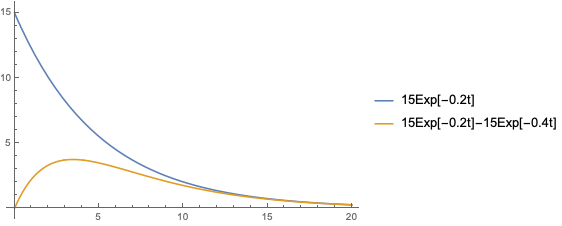
\includegraphics[width=0.8\linewidth]{p6.png} 
\end{center}
\end{example}

\begin{example}
In this example, extracted from problem 5.1.36, we are given the system 
\begin{equation*}
\mathbf{x}' =
\begin{bmatrix}
-\frac{1}{2} & 0 & \frac{1}{2}\\
\frac{1}{2} & -\frac{1}{5} & 0\\
0 & \frac{1}{5} & -\frac{1}{2}
\end{bmatrix} \mathbf{x},
\end{equation*}
with initial condition 
\begin{equation*}
\mathbf{x}(0) =
\begin{bmatrix}
18 \\
0 \\
0
\end{bmatrix}.
\end{equation*}
The characteristic polynomial is 
\begin{equation*}
p(r)=-\frac{9r}{20}-\frac{6r^2}{5}-r^3,
\end{equation*}
with roots $r_1=0, r_2=-\frac{3}{5}+\frac{3i}{10}, r_3=-\frac{3}{5}-\frac{3i}{10}$, and associated eigenvectors
\begin{equation*}
\mathbf{v}_1 =
\begin{bmatrix}
1 \\
\frac{5}{2} \\
1
\end{bmatrix}, \ \mathbf{v}_2 =
\begin{bmatrix}
-\frac{1}{2}-\frac{3i}{2} \\
-\frac{1}{2}+\frac{3i}{2}\\
1
\end{bmatrix}, \ \mathbf{v}_3 =
\begin{bmatrix}
-\frac{1}{2}+\frac{3i}{2} \\
-\frac{1}{2}-\frac{3i}{2}\\
1
\end{bmatrix}.
\end{equation*}
The general solution of the problem can be written in terms of complex exponentials as
\begin{equation*}
\mathbf{x}(t) = C_1
\begin{bmatrix}
1 \\
\frac{5}{2} \\
1
\end{bmatrix}+ C_2e^{-\frac{3t}{5}+\frac{3it}{10}}
\begin{bmatrix}
-\frac{1}{2}-\frac{3i}{2} \\
-\frac{1}{2}+\frac{3i}{2}\\
1
\end{bmatrix}+ C_3e^{-\frac{3t}{5}-\frac{3it}{10}}
\begin{bmatrix}
-\frac{1}{2}+\frac{3i}{2} \\
-\frac{1}{2}-\frac{3i}{2}\\
1
\end{bmatrix}
\end{equation*}
At time $t=0$, we observe 
\begin{equation*}
\begin{bmatrix}
C_1 + C_2\left(-\frac{1}{2}-\frac{3i}{2}\right) + C_3\left(-\frac{1}{2}+\frac{3i}{2}\right) \\
\frac{5C_1}{2} + C_2\left(-\frac{1}{2}+\frac{3i}{2}\right) + C_3\left(-\frac{1}{2}-\frac{3i}{2}\right) \\
C_1 + C_2 + C_3
\end{bmatrix} =
\begin{bmatrix}
18 \\
0 \\
0
\end{bmatrix}
\end{equation*}
By inverting the coefficient matrix (or alternatively, solving it by elimination) we find
\begin{equation*}
\begin{bmatrix}
C_1 \\
C_2 \\
C_3
\end{bmatrix} =
\begin{bmatrix}
4 \\
-2+4i \\
-2-4i
\end{bmatrix},
\end{equation*}
thus we find that 
\begin{equation*}
\mathbf{x}(t) = 4
\begin{bmatrix}
1 \\
\frac{5}{2} \\
1
\end{bmatrix} + (-2+4i)e^{-\frac{3t}{5}+\frac{3it}{10}}
\begin{bmatrix}
-\frac{1}{2}-\frac{3i}{2} \\
-\frac{1}{2}+\frac{3i}{2}\\
1
\end{bmatrix} + (-2-4i)e^{-\frac{3t}{5}-\frac{3it}{10}}
\begin{bmatrix}
-\frac{1}{2}+\frac{3i}{2} \\
-\frac{1}{2}-\frac{3i}{2}\\
1
\end{bmatrix}.
\end{equation*}
By converting complex exponentials into trigonometric functions via Euler's formula, we find the real form of the solution, 
\begin{equation*}
\mathbf{x}(t) = 
\begin{bmatrix}
4 + 2e^{-3t}{5}\left(7\cos\left(\frac{3t}{10}\right) -2\sin\left(\frac{3t}{10}\right)\right) \\
10 -10e^{\frac{-3t}{5}}\left(\cos(\left(\frac{3t}{10}\right)-\sin\left(\frac{3t}{10}\right) \right) \\
4 - 4e^{\frac{3t}{5}}\left(\cos(\left(\frac{3t}{10}\right) -2\sin\left(\frac{3t}{10}\right) \right)
\end{bmatrix}
\end{equation*}
The limiting amounts of salt in each tank are 
\begin{equation*}
\lim_{t \to \infty} x_1(t) = 4,\   \lim_{t \to \infty} x_1(t) = 10, \ \lim_{t \to \infty} x_3(t) = 4.
\end{equation*} 
Below is a comparative plot of the graphs of the solutions
\begin{center}
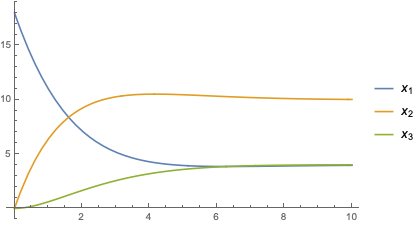
\includegraphics[width=0.8\linewidth]{p7.png} 
\end{center}
\end{example}

\section*{Section 5.4: Second-Order Systems and Mechanical Applications.}
In section 5.4 we discuss mechanical systems described by second-order systems of type 
\begin{equation*}
M\mathbf{x}^{'} = K\mathbf{x},
\end{equation*}
where $M$ is a diagonal matrix describing the masses of the system, while $K$ is called the stiffness matrix, and encodes the resulting spring constants. For simplicity, we assume that the matrix $A=M^{-1}K$ has only negative eigenvalues. 

\begin{example}
Consider the following system, extracted from problem 5.4.4, we are given masses $m_1=m_2=1$, and stiffness matrix
\begin{equation*}
K =
\begin{bmatrix}
-3 & 2 \\
2 & -3
\end{bmatrix}
\end{equation*}
The characteristic equation for this problem is 
\begin{equation*}
r^2+6r+5= 0,
\end{equation*}
with roots $r_1=-5, r_2=-1$, and associated eigenvectors
\begin{equation*}
\mathbf{v}_1 = 
\begin{bmatrix}
-1\\
1
\end{bmatrix}, \ \mathbf{v}_2 =
\begin{bmatrix}
1\\
1
\end{bmatrix}
\end{equation*}
Solutions can thus be written as
\begin{equation*}
x(t) =\begin{bmatrix}
-C_1\cos(\sqrt{5}t) - C_2 \sin(\sqrt{5}t) \\
C_1\cos(\sqrt{5}t)+C_2\sin(\sqrt{5}t)
\end{bmatrix} + 
\begin{bmatrix}
C_3\cos(t) + C_4\sin(t) \\
C_3\cos(t) + C_4\sin(t) 
\end{bmatrix}
\end{equation*}
\end{example}

\begin{thebibliography}{0}

\bibitem{EdPeCa} C. Henry Edwards, David E. Penney and David T. Calvis, {\it Differential Equations and Boundary Value Problems: Computing and Modelling}, 5th edition, Pearson, 2014.

\end{thebibliography}
\end{document}


